% This is text associated with the open textbook "Open Electromagnetics"
% See immediately below for author, date
% This work is licensed under the Creative Commons Attribution-ShareAlike 4.0 International License. (CC BY-SA 4.0) 
% To view a copy of the license, visit http://creativecommons.org/licenses/by-sa/4.0/

%ORB TITLE Capacitance
%ORB AUTHOR 0        # S.W. Ellingson, Virginia Tech (ellingson@vt.edu)
%ORB DATE 20180806   # yyyymmdd
%ORB ABSTRACT Capacitance

\label{m0112_Capacitance} % <-- Must match name of this file and module directory name.  Don't mess with this!
\index{capacitance|(}

When separate regions of positive and negative charge exist in proximity, Coulomb forces (Section~\ref{m0102_Coulombs_Law}) will attempt to decrease the separation between the charges.
As noted in Section~\ref{m0061_Force_Energy_and_Potential_Difference}, this can be interpreted as a tendency of a system to reduce its potential energy.
If the charges are fixed in place, then the potential energy remains constant.  
This potential energy is proportional to the Coulomb force.
Referring back to Section~\ref{m0102_Coulombs_Law}, the Coulomb force is:
%
\begin{itemize}
\item Proportional to quantity of positive charge squared  
\item Inversely proportional to the separation between the charges squared
\item Inversely proportional to the permittivity of the material separating the charges
\end{itemize}
Therefore, the potential energy of the system is likewise dependent on charge, separation, and permittivity.
Furthermore, we see that the ability of a system to store energy in this manner depends on the geometry of the charge distribution and the permittivity of the intervening material.  

Now recall that the electric field intensity ${\bf E}$ 
\index{electric field intensity}
is essentially defined in terms of the Coulomb force; 
\index{force}
i.e., ${\bf F}=q{\bf E}$ (Section~\ref{m0002_Electric_Field_Intensity}).
So, rather than thinking of the potential energy of the system as being associated with the Coulomb force, it is equally valid to think of the potential energy as being stored in the electric field associated with the charge distribution.
It follows from the previous paragraph that the energy stored in the electric field depends on the geometry of the charge distribution and the permittivity of the intervening media.  
This relationship is what we mean by \emph{capacitance}.
We summarize as follows:
%
%ORB HIGHLIGHT
\begin{mdframed}[backgroundcolor=yellow!20,nobreak=true] 
Capacitance 
\index{capacitance!definition}
is the ability of a structure to store energy in an electric field.
\end{mdframed}
%
and
%
%ORB HIGHLIGHT
\begin{mdframed}[backgroundcolor=yellow!20,nobreak=true] 
The capacitance of a structure depends on its geometry and the permittivity of the medium separating regions of positive and negative charge.
\end{mdframed}

Note that capacitance does \emph{not} depend on charge, which we view as either a stimulus or response from this point of view.
The corresponding response or stimulus, respectively, is the potential associated with this charge.
This leads to the following definition:
%
\begin{equation}
\boxed{
C \triangleq \frac{Q_+}{V}
}
\label{m0112_Cdef}
\end{equation} 
%
where $Q_+$ (units of C) is the total positive charge, $V$ (units of V) is the potential associated with this charge (defined such that it is positive),  and $C$ (units of F) is the associated capacitance. So:
%
%ORB HIGHLIGHT
\begin{mdframed}[backgroundcolor=yellow!20,nobreak=true] 
In practice, capacitance is defined as the ratio of charge present on one conductor of a two-conductor system to the potential difference between the conductors (Equation~\ref{m0112_Cdef}). 
\end{mdframed}
%
In other words, a structure is said to have greater capacitance if it stores more charge -- and therefore stores more energy -- in response to a given potential difference.

Figure~\ref{m0112_fGenericCap} shows the relevant features of this definition.
Here, a battery imposes the potential difference $V$ between two regions of perfectly-conducting material.
$Q_+$ is the total charge on the surface of the PEC region attached to the positive terminal of the battery.
An equal amount of negative charge appears on the surface of the PEC region attached to the negative terminal of the battery (Section~\ref{m0025_Charge_and_Electric_Field_for_a_Perfectly_Conducting_Region}).
This charge distribution gives rise to an electric field.
Assuming the two PEC regions are fixed in place, $Q_+$ will increase linearly with increasing $V$, at a rate determined by the capacitance $C$ of the structure. 
%
\begin{figure}
\begin{center}
\pdftooltip{{  % note double braces
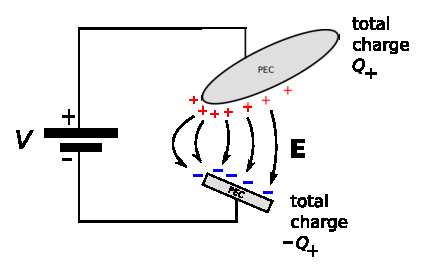
\includegraphics[width=2.5in]{modules/m0112_fGenericCap.eps}
}}{The figure shows a battery with each side connected to a distinct arbitrary, grey region labeled PEC. The regions are parallel. The upper shape is attached to the positive end of the battery has a total charge Q super +. The lower shape is attached to the negative end, with a total charge -Q super +. In the space between the two shapes is an electric field pointing from the upper shape (positive) to the lower shape (negative), labeled E.}
\end{center} 
%\centerline{\scriptsize 
%\copyright~\hyperref[m0112_fGenericCap_Credit]{author} 
%\href{https://creativecommons.org/licenses/by-sa/4.0/}{CC BY~SA 4.0} 
%} 
\caption{
\label{m0112_fGenericCap}
Electrostatic interpretation of capacitance.
}
\end{figure}

\index{capacitor|(}

A \emph{capacitor} is a device that is designed to exhibit a specified capacitance.
We can now make the connection to the concept of the capacitor as it appears in elementary circuit theory.
In circuit theory, the behavior of devices is characterized in terms of terminal voltage $V_T$ in response to terminal current $I_T$, and vice versa.
First, note that current does not normally flow through a capacitor,\footnote{If it does, it's probably experiencing \emph{dielectric breakdown}; see Section~\ref{m0109_Dielectric_Breakdown}.} so when we refer to ``terminal current'' for a capacitor, what we \emph{really} mean is the flow of charge arriving or departing from one of the conductors via the circuit, which is equal to the flow of charge departing or arriving (respectively) at the other conductor.  This gives the appearance of current flow through the capacitor when the current is examined from outside the capacitor.
With that settled, we proceed as follows.
Using Equation~\ref{m0112_Cdef}, we express the voltage $V_T$ across the terminals of a capacitor having capacitance $C$:
%
\begin{equation}
V_T = \frac{Q_+}{C}
\end{equation}
%
We seek a relationship between $V_T$ and $I_T$.
Current is charge per unit time, so the charge on either conductor is the integral of $I_T$ over time; i.e.:
%
\begin{equation}
Q_+(t) = \int_{t_0}^{t} { I_T(\tau)~d\tau } + Q_+(t_0)
\end{equation}
%
where $t_0$ is an arbitrarily-selected start time.
In other words, amps integrated over time is charge. If we define $I_T$ as being positive in the direction of the flow of positive charge as is the usual convention, then we have:
%
\begin{equation}
V_T(t) = \frac{1}{C}\int_{t_0}^{t} { I_T(\tau)~d\tau } + \frac{1}{C}Q_+(t_0)
\end{equation}
%
Again applying Equation~\ref{m0112_Cdef}, we see that the second term is simply $V_T(t_0)$.
This is the expected relationship from elementary circuit theory.

Finally, solving for $I_T$ we obtain the differential form of this relationship:
%
\begin{equation}
I_T(t) = C\frac{d}{dt}V_T(t)
\end{equation}

\index{capacitor|)}

%%%%%%%%%%%%%%%%%%%%%%%%%%%%%%%%%%%%%%%%%%%%

{\bf Additional Reading:}
\begin{itemize}
\item ``\href{https://en.wikipedia.org/wiki/Capacitance}{Capacitance}'' on Wikipedia.
\item ``\href{https://en.wikipedia.org/wiki/Capacitor}{Capacitor}'' on Wikipedia.
\end{itemize}

\index{capacitance|)}
